\documentclass[useAMS,usenatbib]{mn2e}

\usepackage{multicol}
\usepackage[english]{babel}
\usepackage{graphicx}
\usepackage{epsfig}
\usepackage{natbib}
\usepackage{times}
\usepackage{ulem}
\usepackage{array}
\usepackage[T1]{fontenc}
%\usepackage[section] {placeins}
\bibliographystyle{mn2e}
\citestyle{mn2e}


%%%%%%%% Begin custom definitions %%%%%%%%%%%%%
\usepackage{float}
\usepackage{caption}
\input macros.tex
\voffset=-1.4cm
\graphicspath{{./plots/}}
%%%%%%%% End custom definitions %%%%%%%%%%

\begin{document}

\title[Seed Black Holes in the First Galaxies]{The Dynamics of Seed
  Black Holes in the First Galaxies}

\author[C. Shi et al.]{Chao Shi$^1$\thanks{e-mail:
    cshi31@gatech.edu}, John H. Wise$^1$, Other authors\\
  $^{1}$ Center for Relativistic Astrophysics, Georgia Institute of
  Technology, 837 State Street, Atlanta, GA
  30332, USA\\
}
\pagerange{\pageref{firstpage}--\pageref{lastpage}} \pubyear{2015}

\maketitle
\label{firstpage}

\begin{abstract}

  \textbf{Copied from AAS.  Should be updated before submission with
    main results.} The discovery of bright quasars at redshift $z \ge
  6$ in the Sloan Digital Sky Survey implies that black holes (BHs) as
  massive as $10^9 \Ms$ were already assembled within 1
  Gyr. Generically, these SMBHs are thought to have assembled by
  mergers with other BHs and by gas accretion onto less massive seed
  BHs. One candidate of such seed BHs are Population III (Pop III)
  stellar remnants. In order to map out plausible scenarios such
  massive objects form from Pop III remnants, we run a cosmological
  adaptive refinement mesh simulation of an overdense region of about
  300 Mpc$^3$, which forms a few $10^9 \Ms$ dark matter halos and over
  13000 Pop III stars by redshift 15. Then we focus on one of these
  massive halos, containing 20 Pop III stellar remnants, to study the
  dynamical behavior of these BH seed candidates. Here we report on
  the evolution of the orbital properties of stellar-mass seed BHs in
  one of the first galaxies. They are distributed throughout the halo,
  creating a swarm of BHs, gradually falling toward the halo center
  through dynamical friction. From these characteristics, we estimate
  the BH merger rate in this particular galaxy, which is an important
  quantity to assess during the early buildup of massive BHs.

\end{abstract}

\begin{keywords}
  galaxies: formation -- galaxies: dwarf -- galaxies: high-redshift --
  methods: numerical
\end{keywords}

\section{Motivation}

\section{Methods}
 
\subsection{Simulation Setup}

\subsection{Orbital Elements}

\section{Results}

\subsection{Stacked Analysis}
Radial distribution of seed BHs at different stages:
\begin{minipage}{\linewidth}
\makebox[\linewidth]{ 
  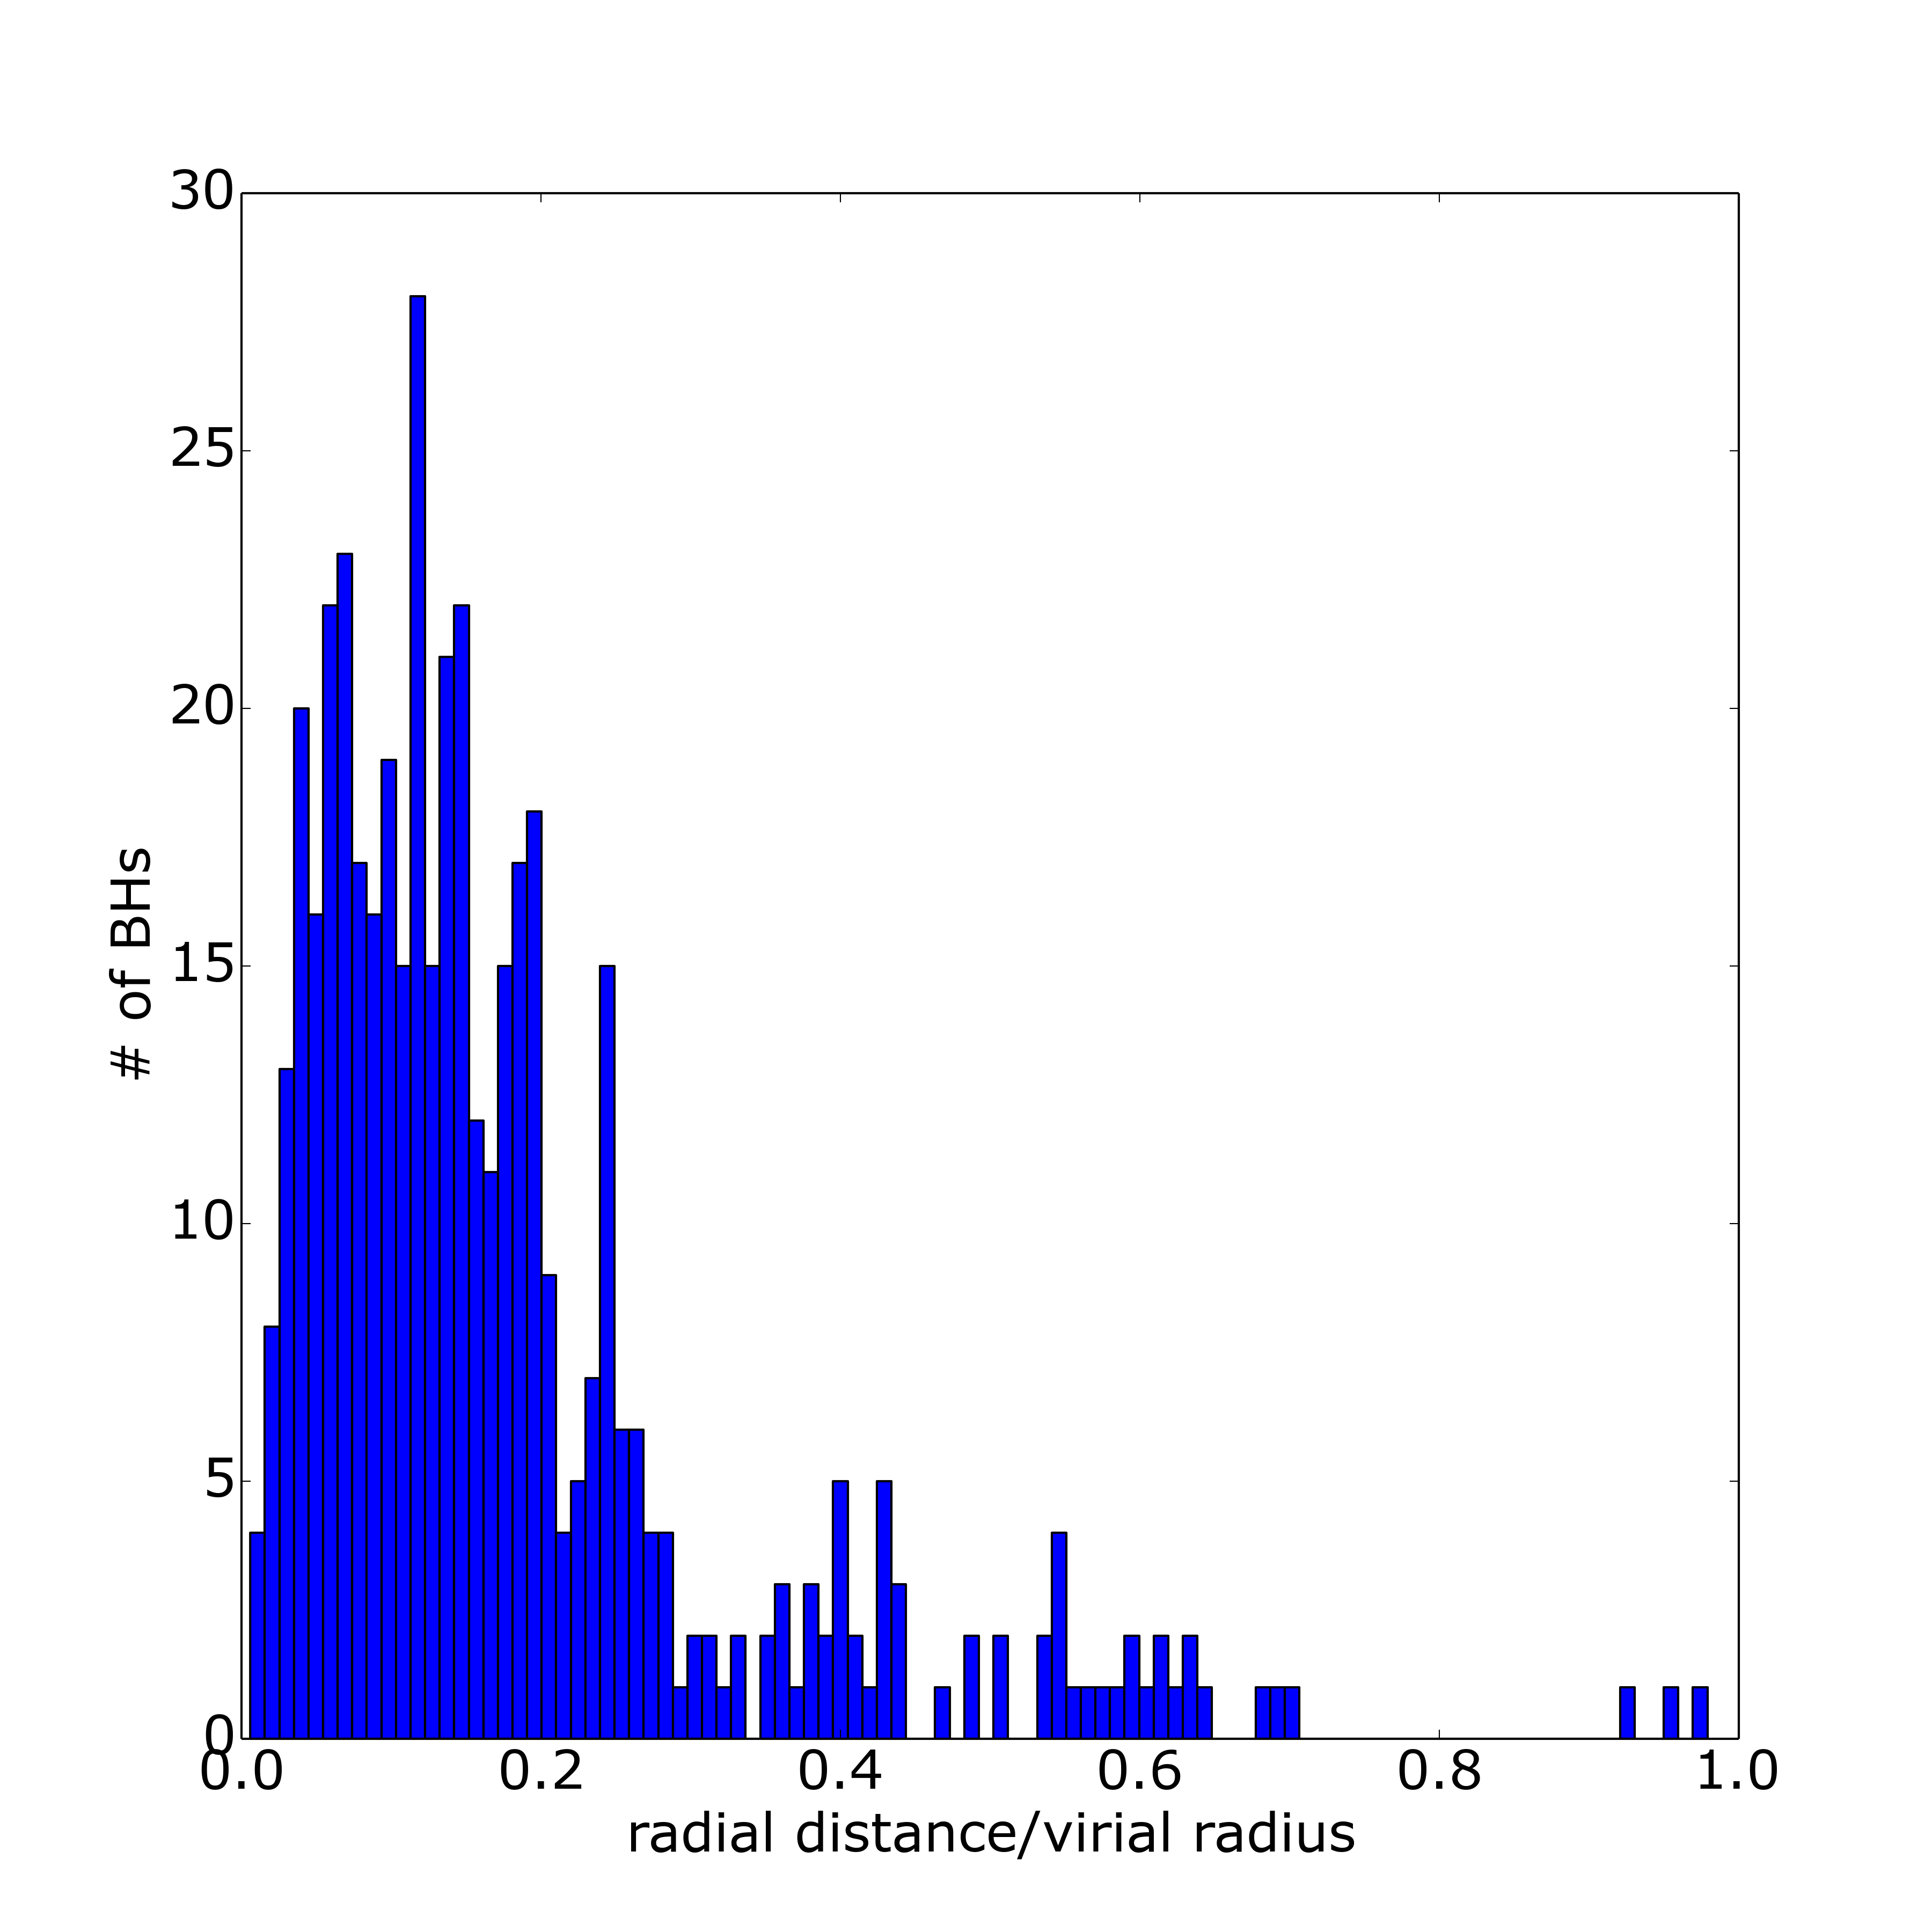
\includegraphics[keepaspectratio=true,width=0.8\linewidth]{rad_dist3.png}
}
\end{minipage}
\begin{figure}
  \centering
  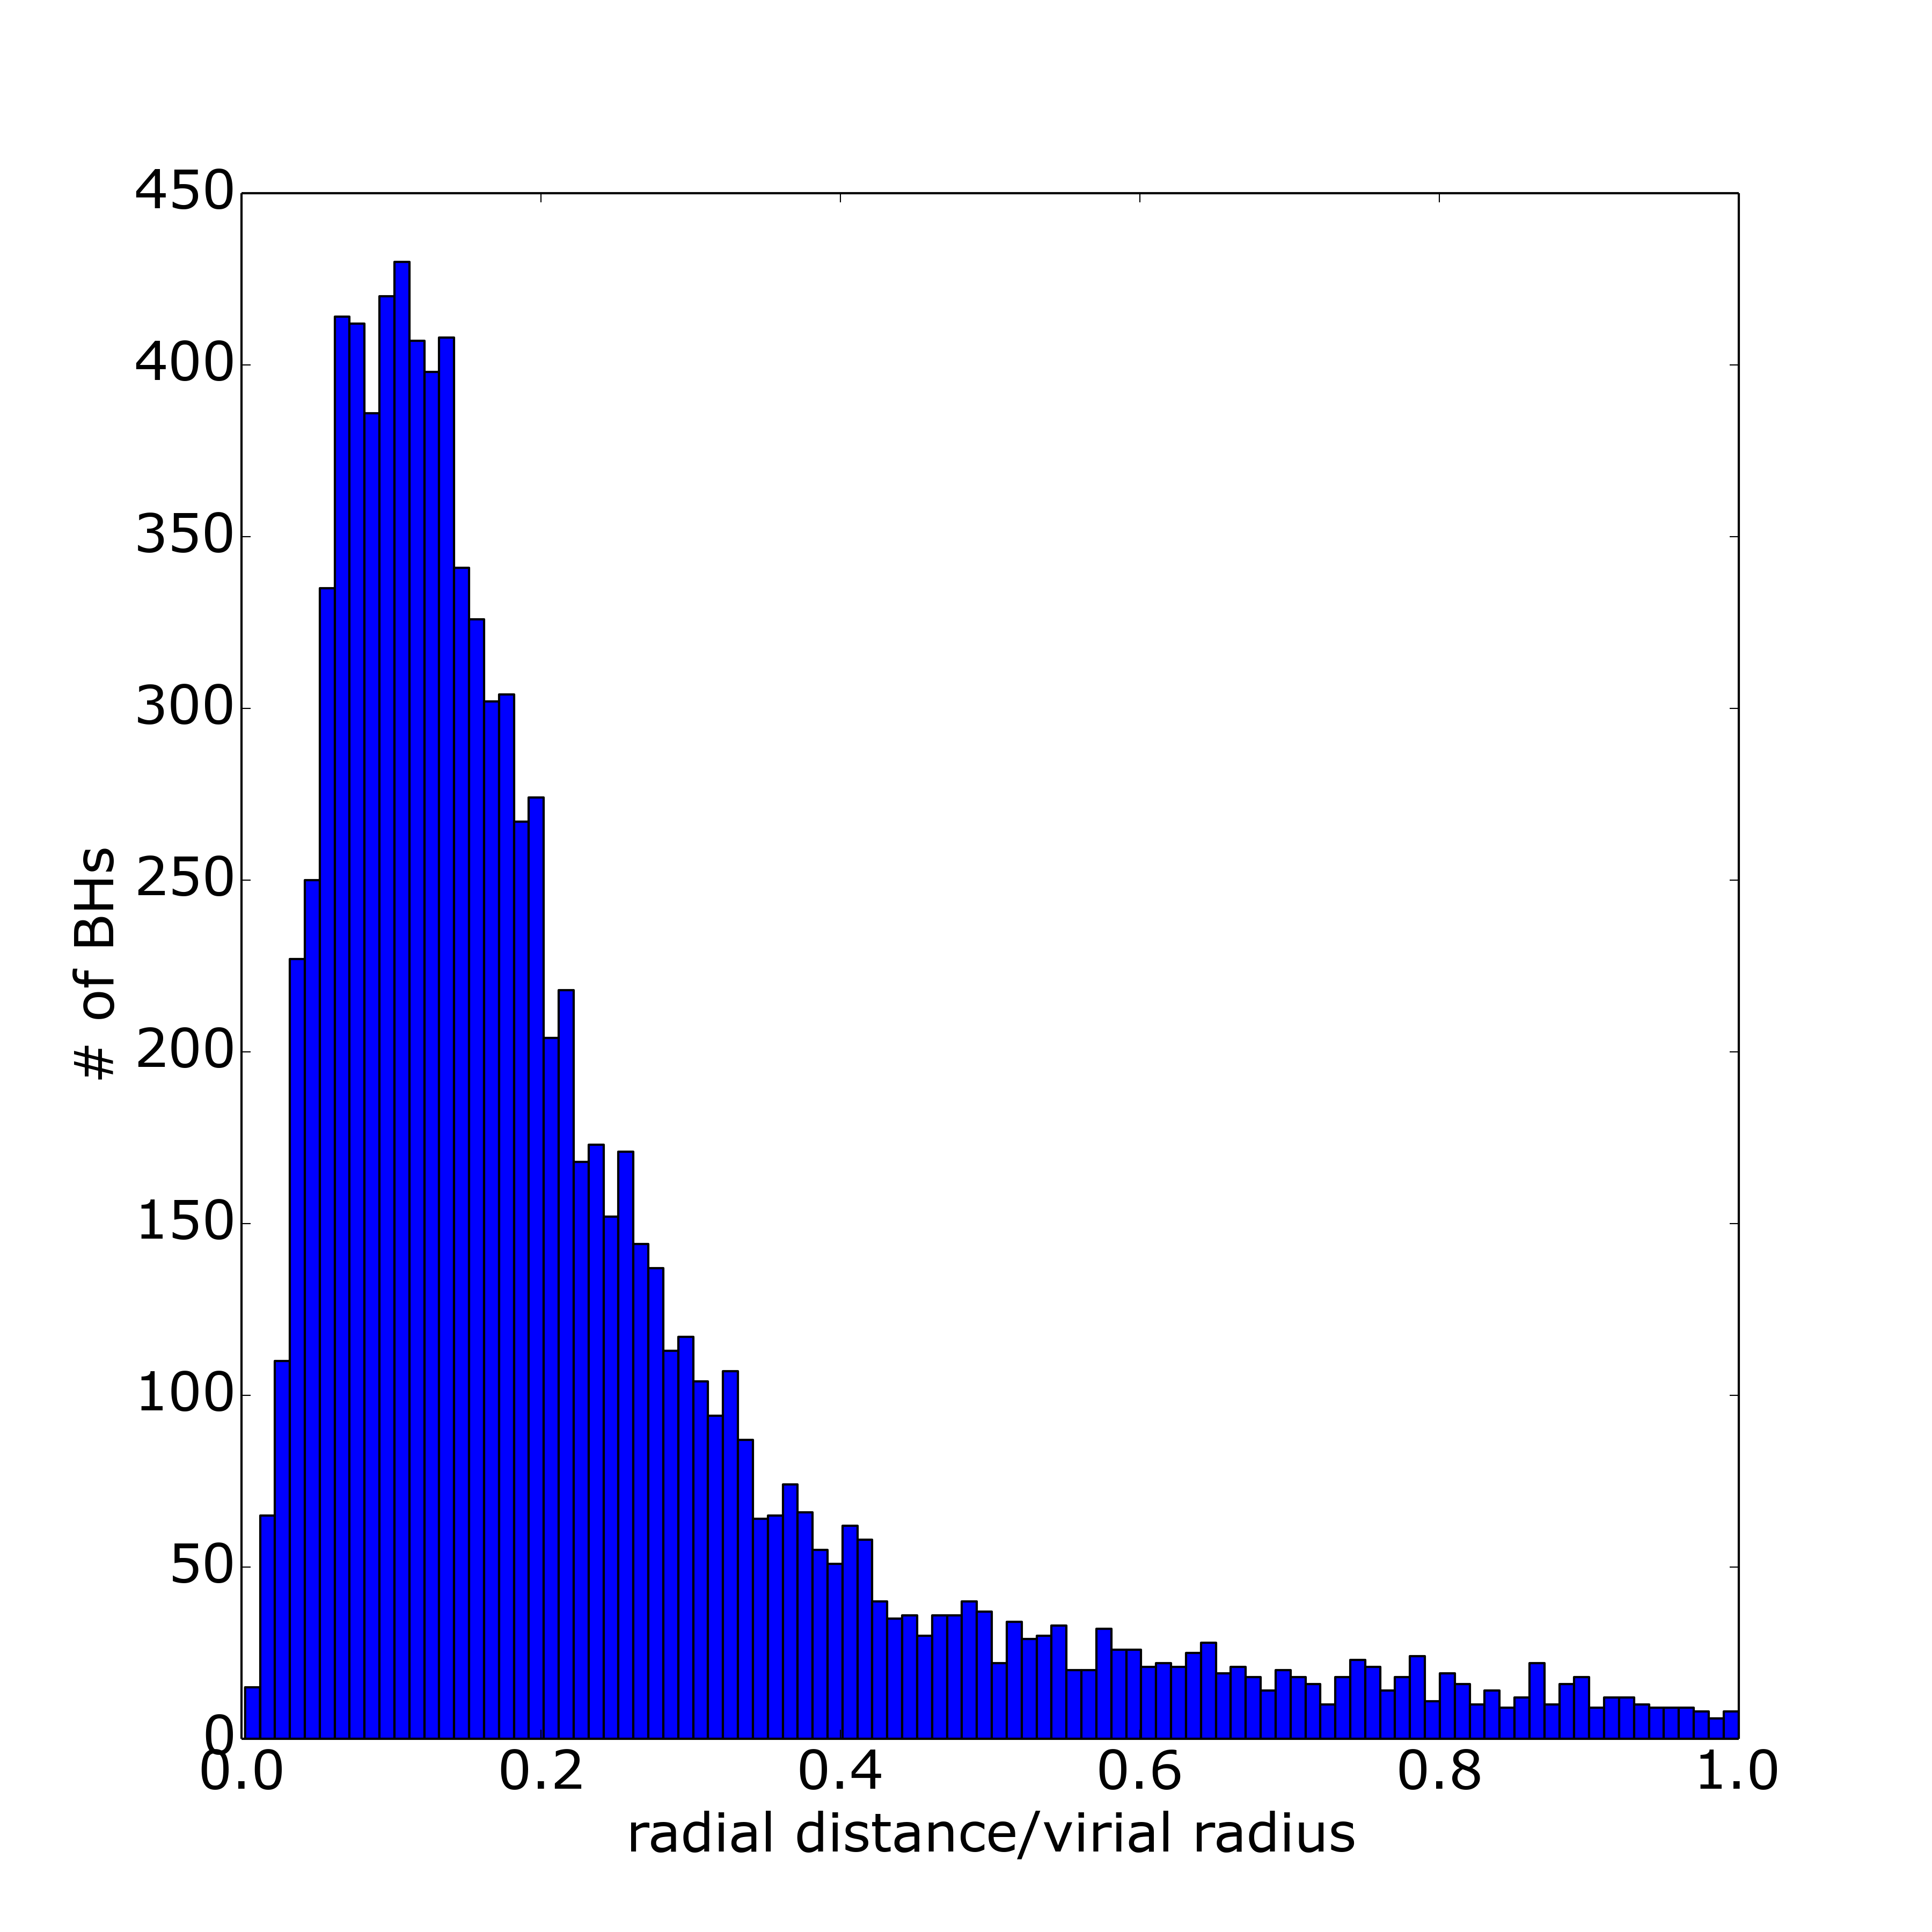
\includegraphics[width=0.8\columnwidth]{rad_dist14.png}
\end{figure}
\begin{figure}
  \centering
  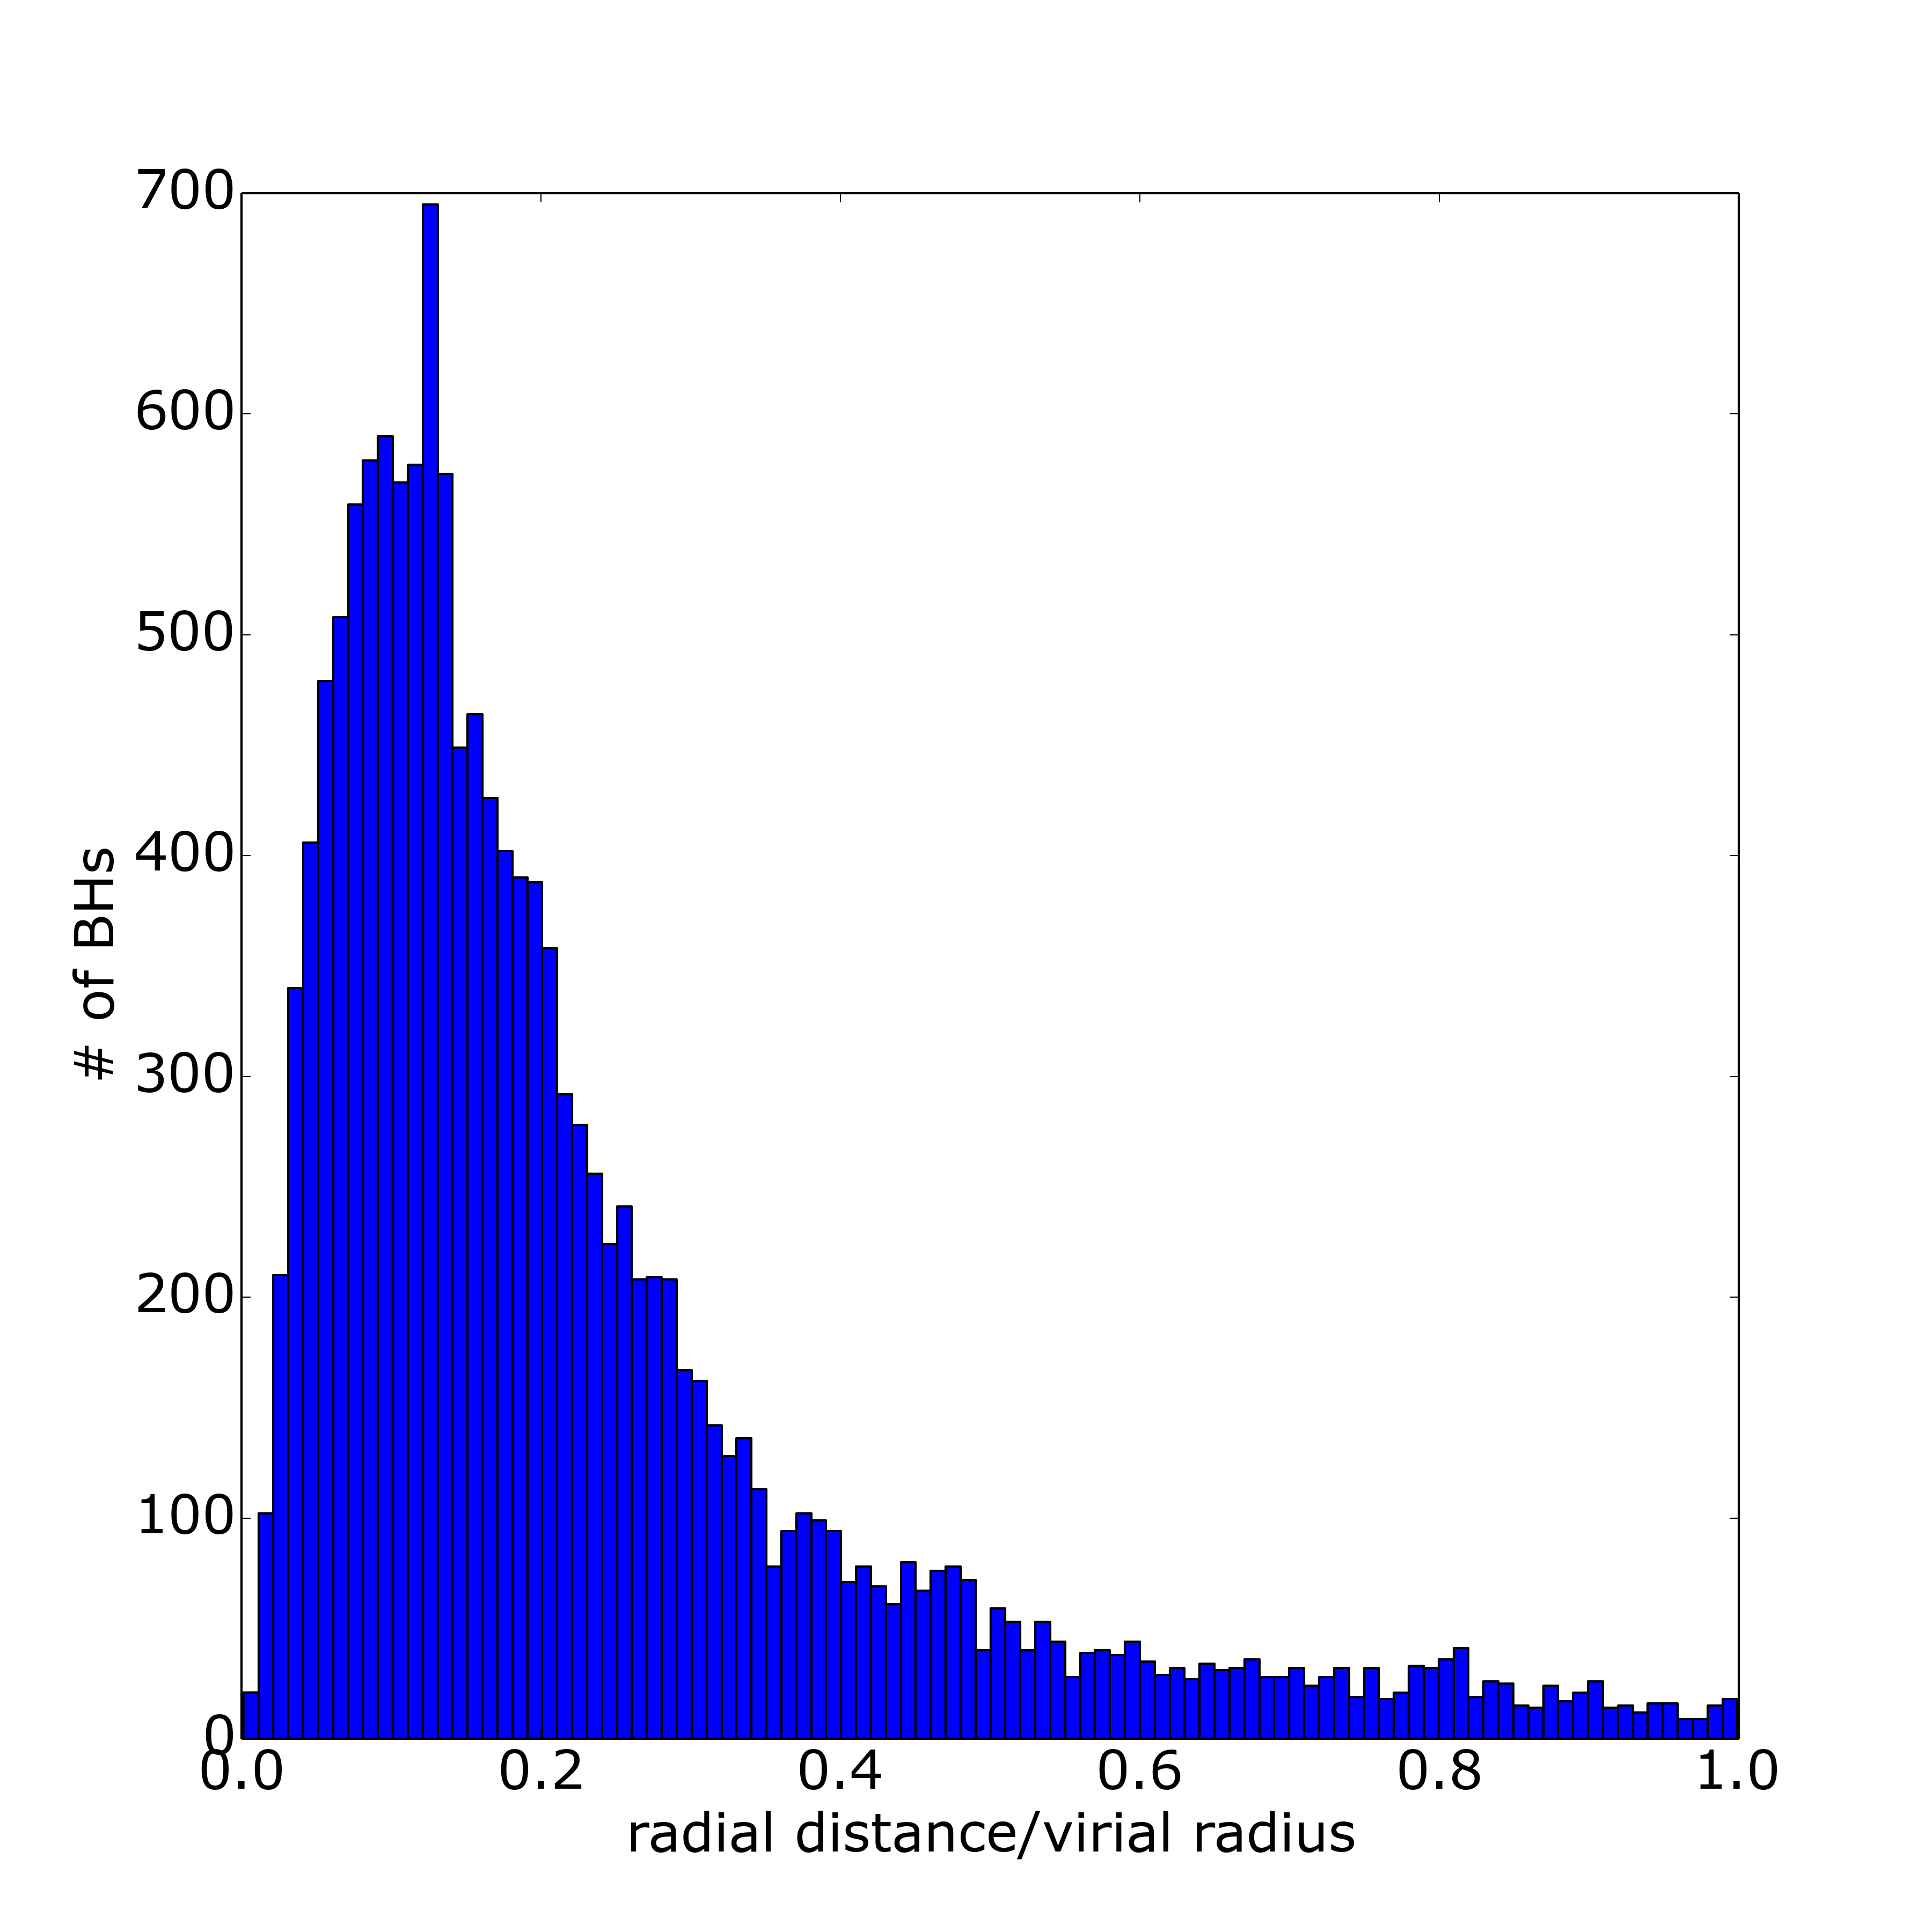
\includegraphics[width=0.8\columnwidth]{rad_dist22.png}
\end{figure}
Radial distribution of seed BHs of the final time step in different mass ranges:
\begin{figure}
  \centering
  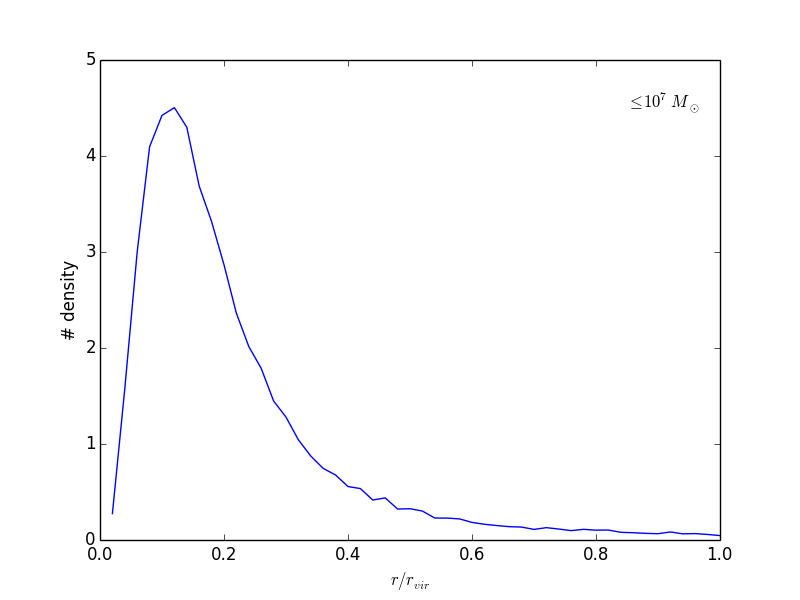
\includegraphics[width=0.8\columnwidth]{radist_mass7.png}
\end{figure}

\begin{figure}
  \centering
  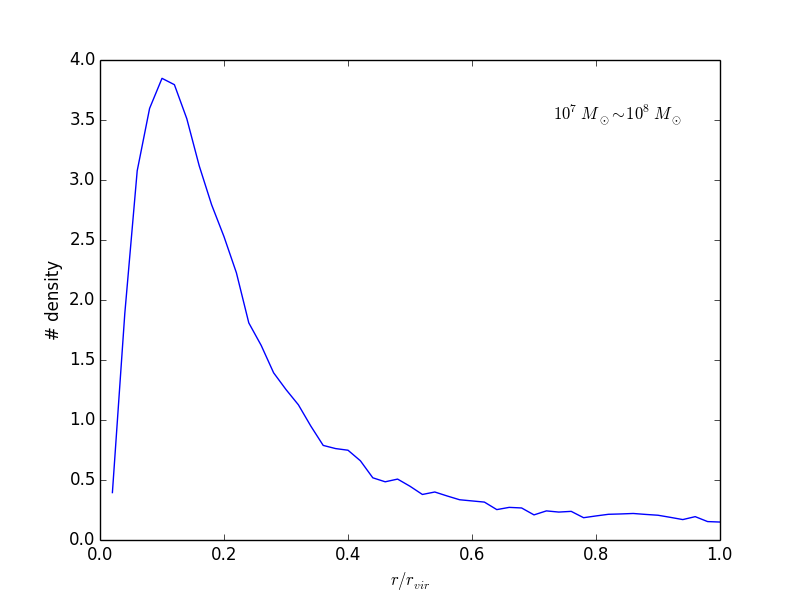
\includegraphics[width=0.8\columnwidth]{radist_mass8.png}
\end{figure}

\begin{figure}
  \centering
  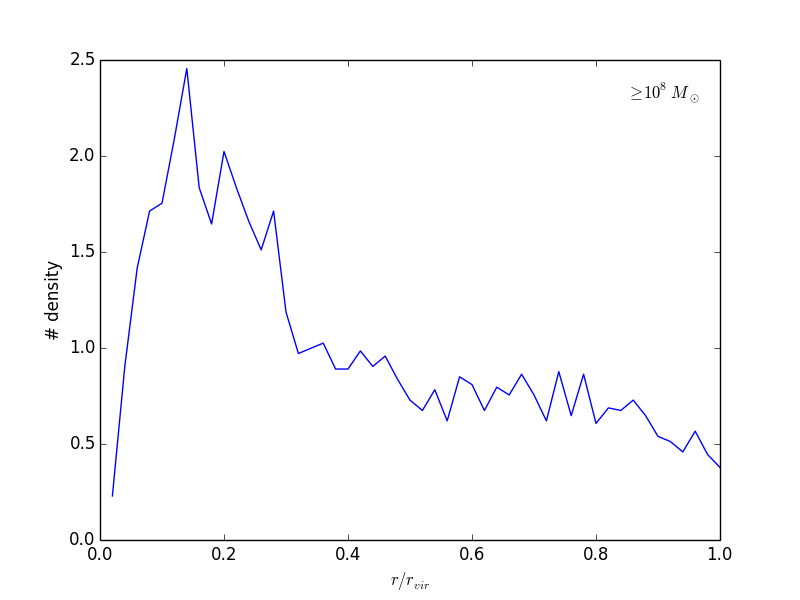
\includegraphics[width=0.8\columnwidth]{radist_mass9.png}
\end{figure}

Orbital properties:
\begin{figure}
  \centering
  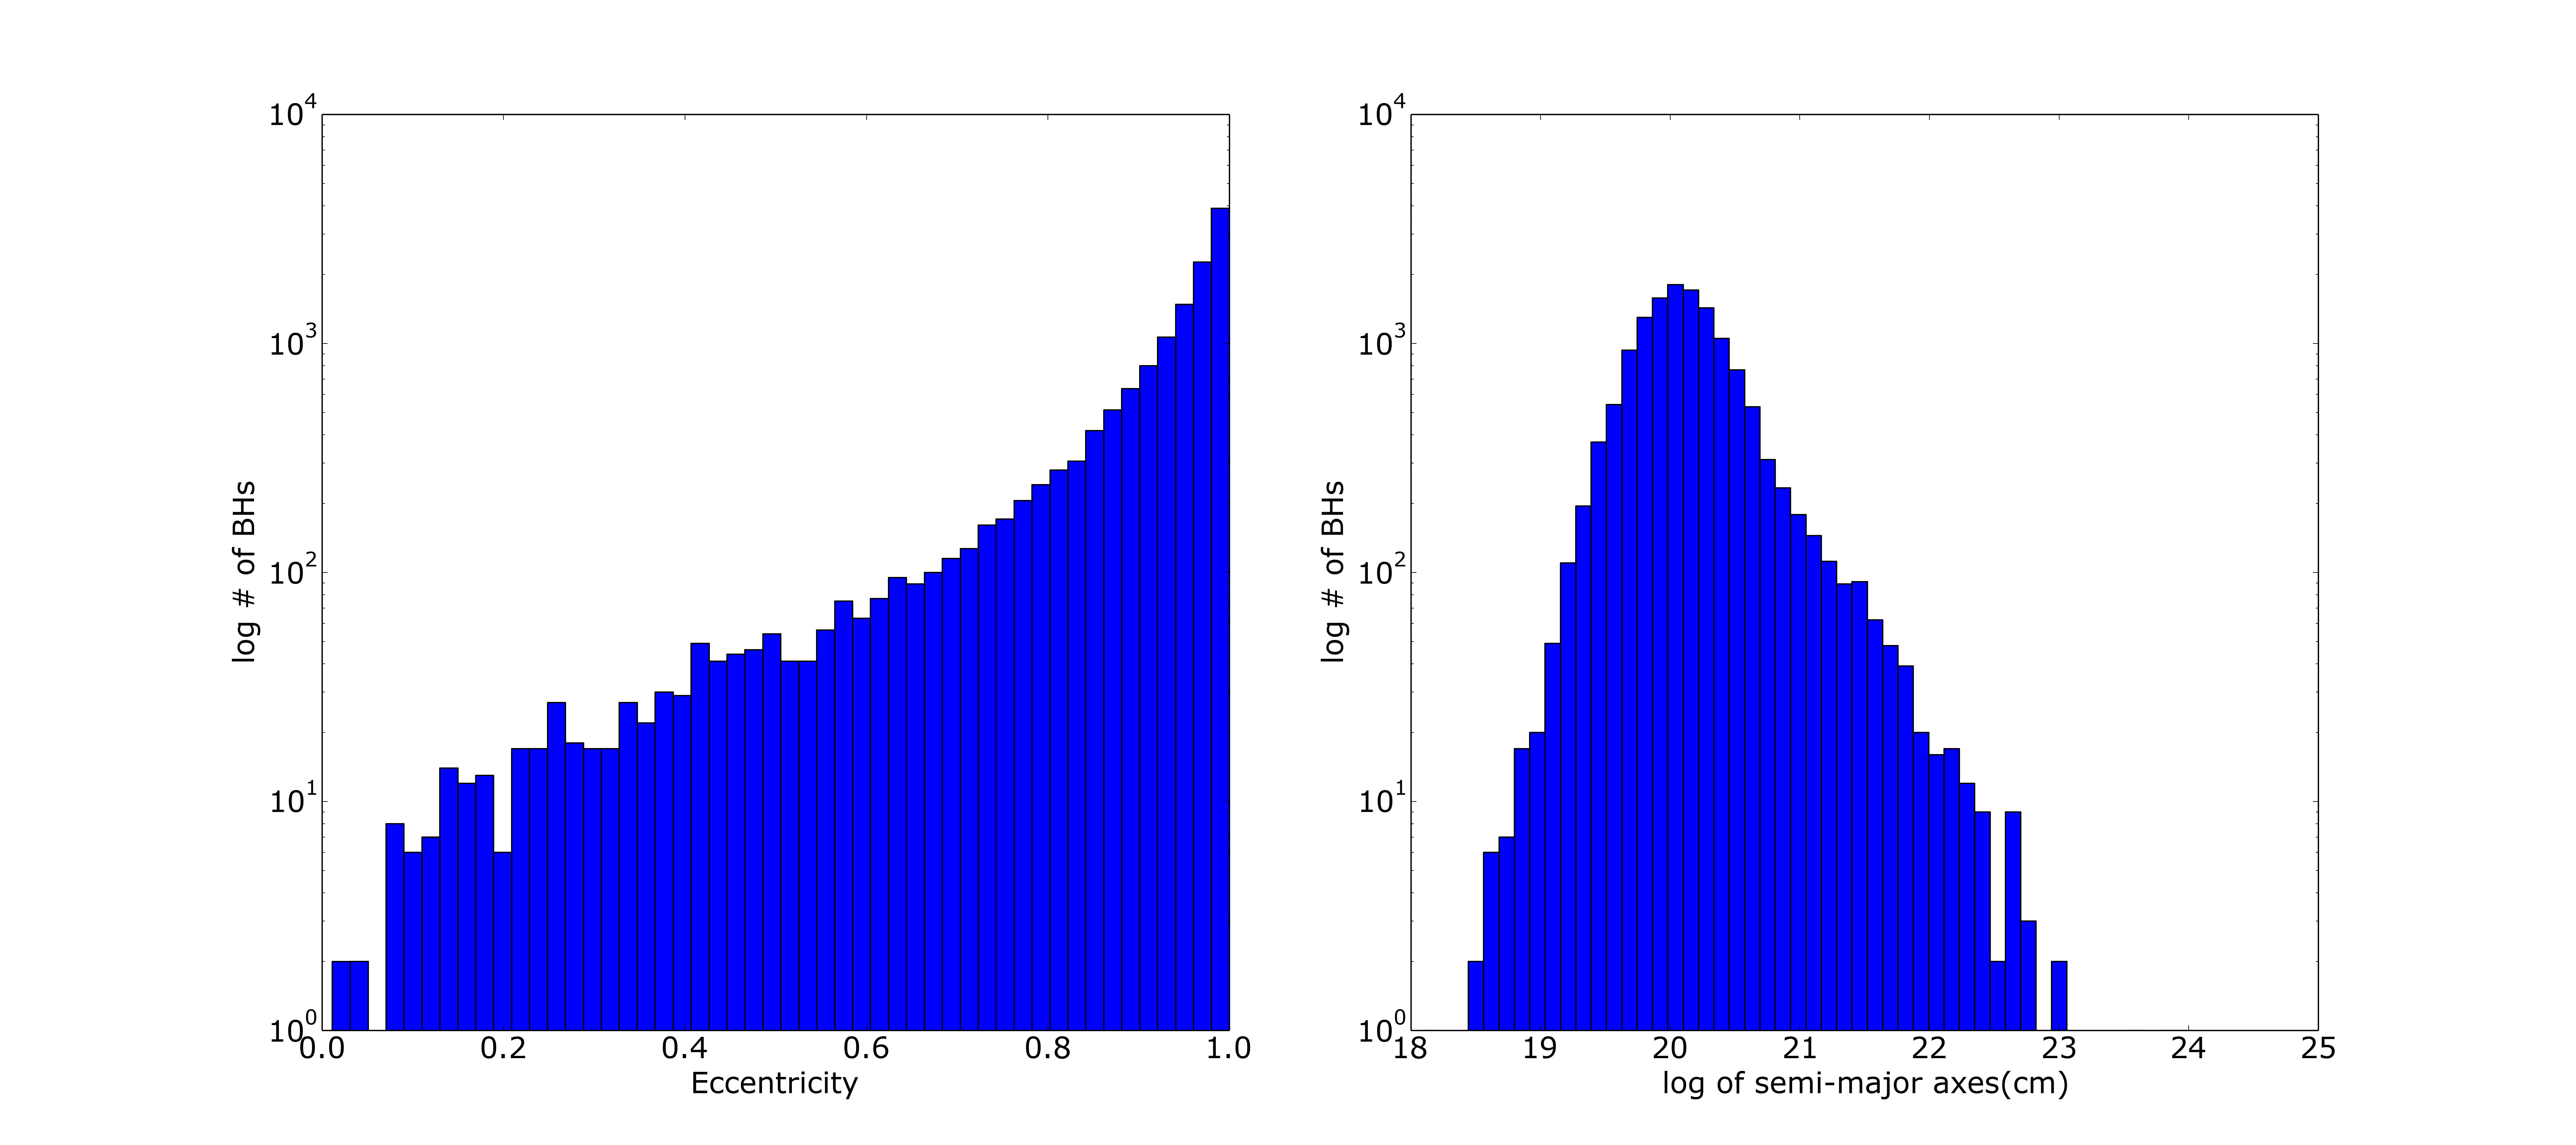
\includegraphics[width=0.8\columnwidth]{bhsorb_new.png}
\end{figure}



\subsection{Case Study: High Temporal Analysis of a Single Galaxy}

Seed BHs position:
\begin{figure}
  \centering
  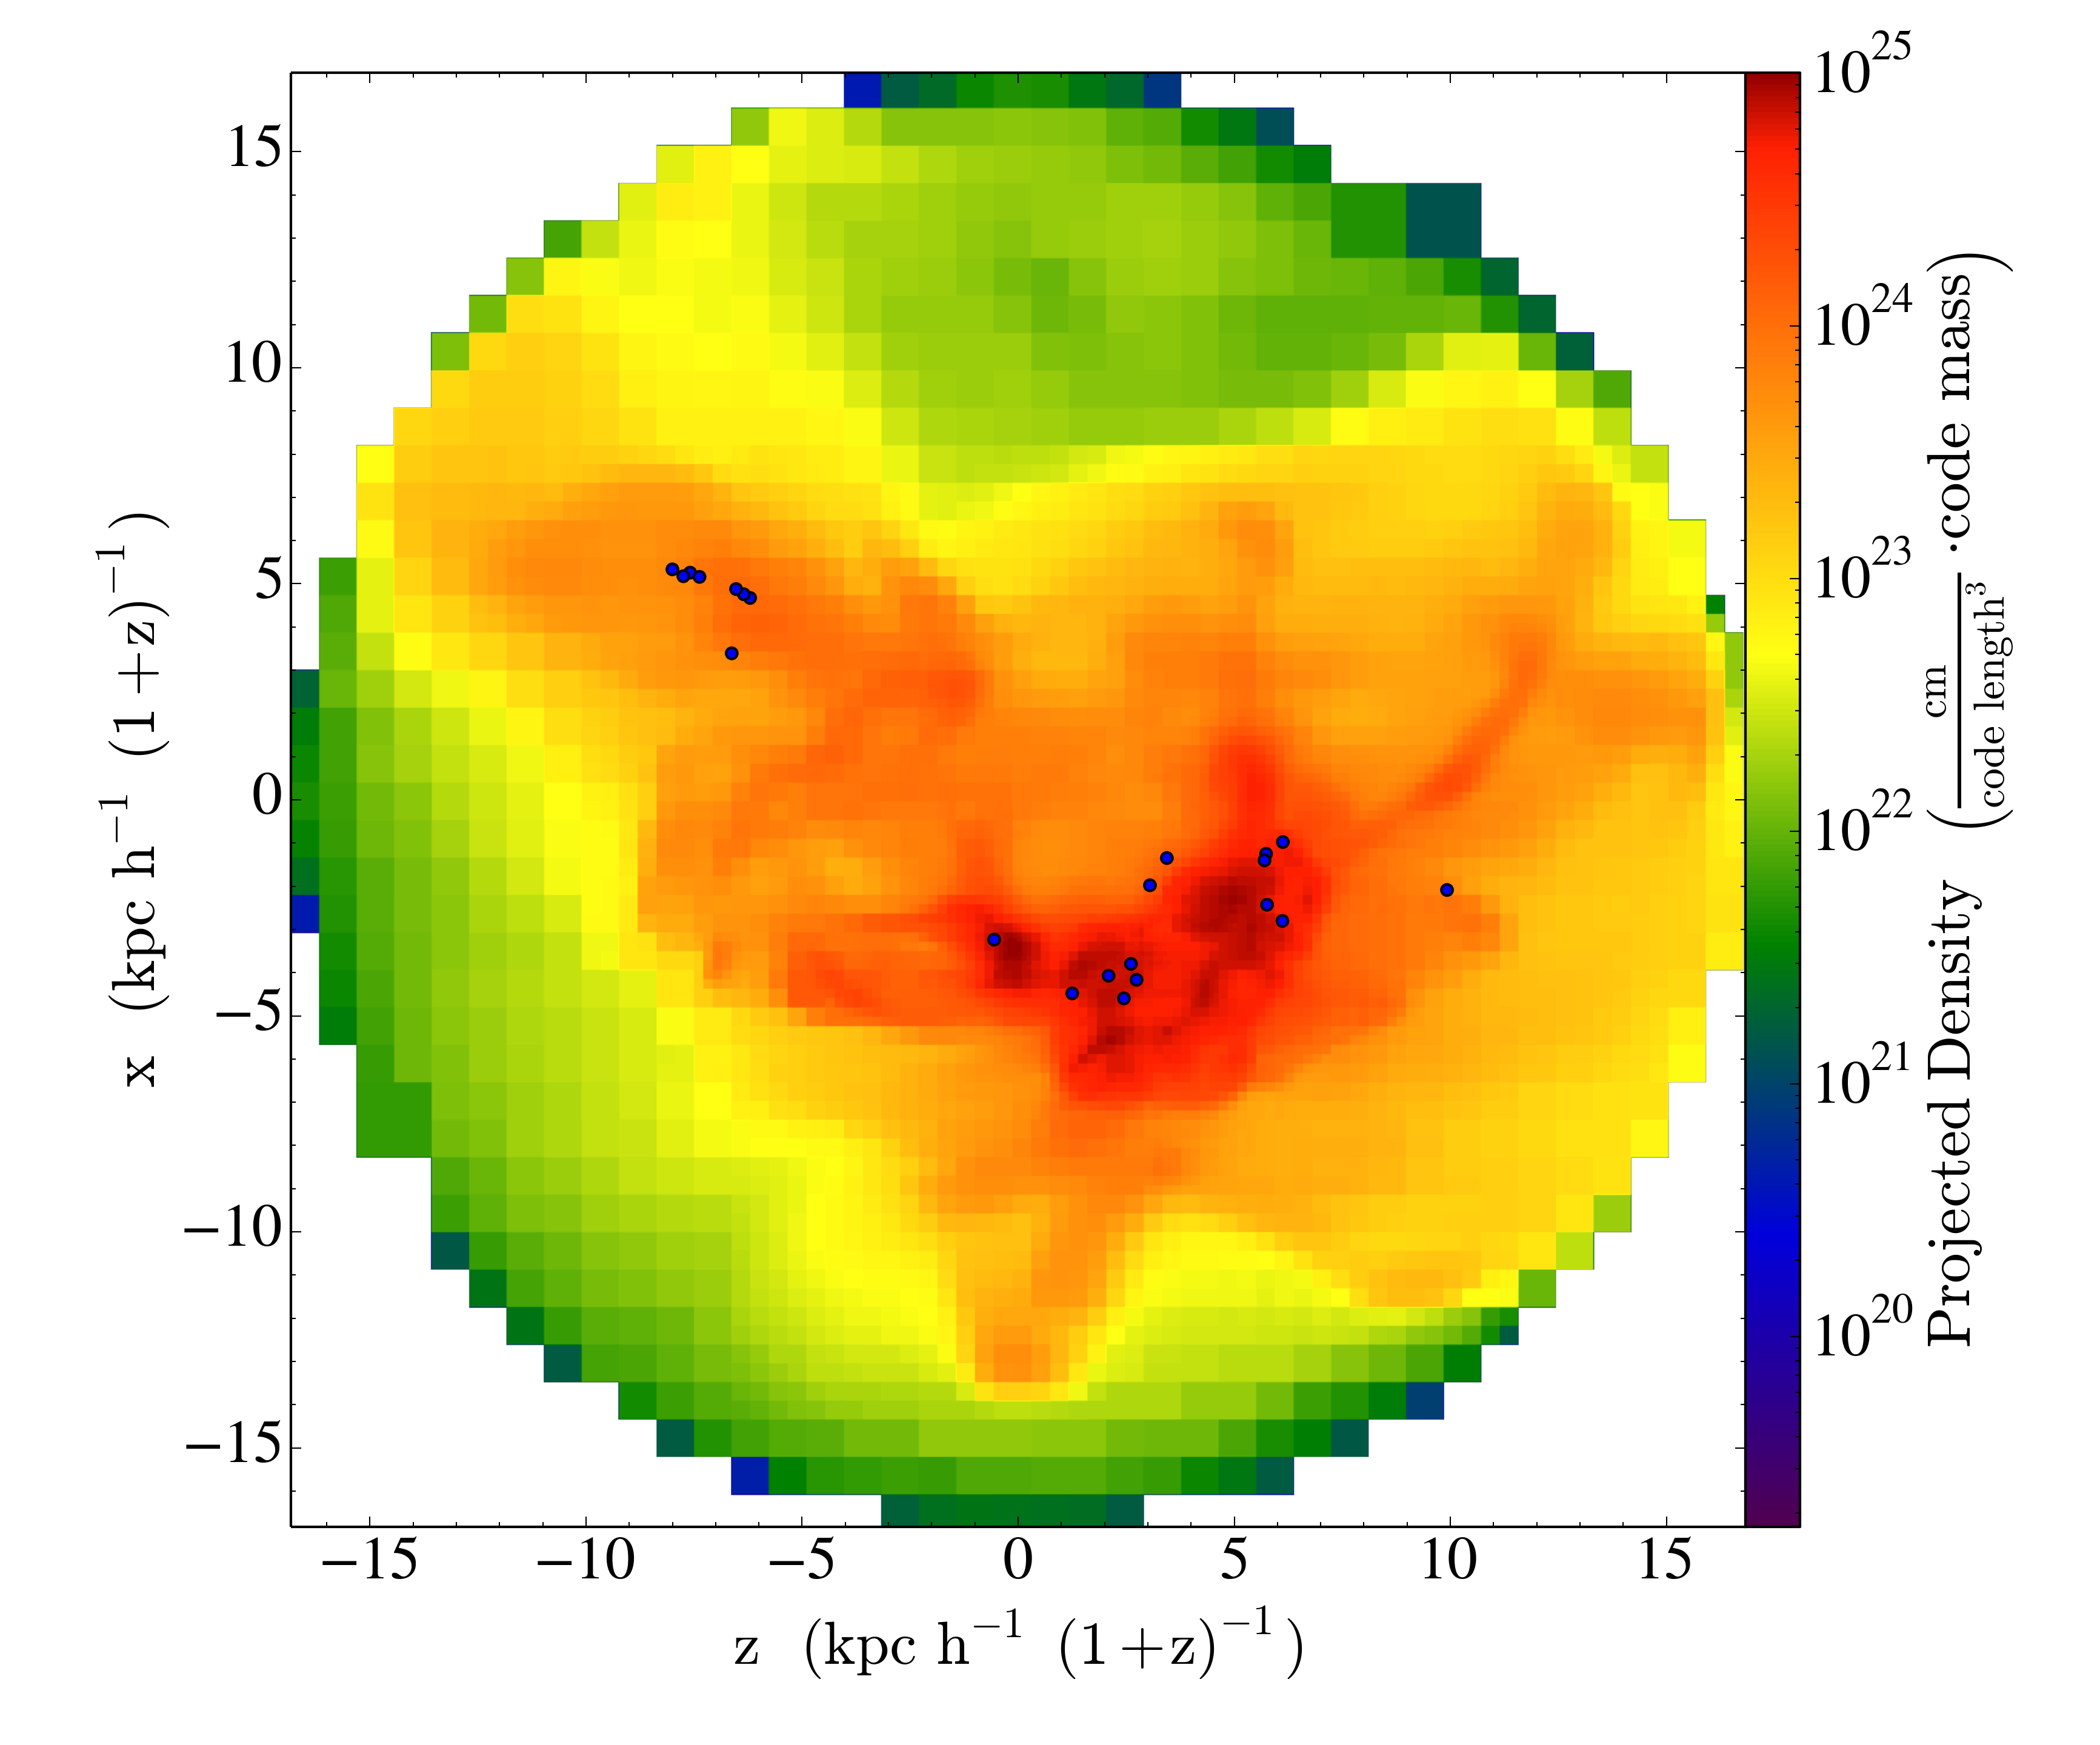
\includegraphics[width=0.8\columnwidth]{P0173_y_D.png}
\end{figure}

\begin{figure}
  \centering
  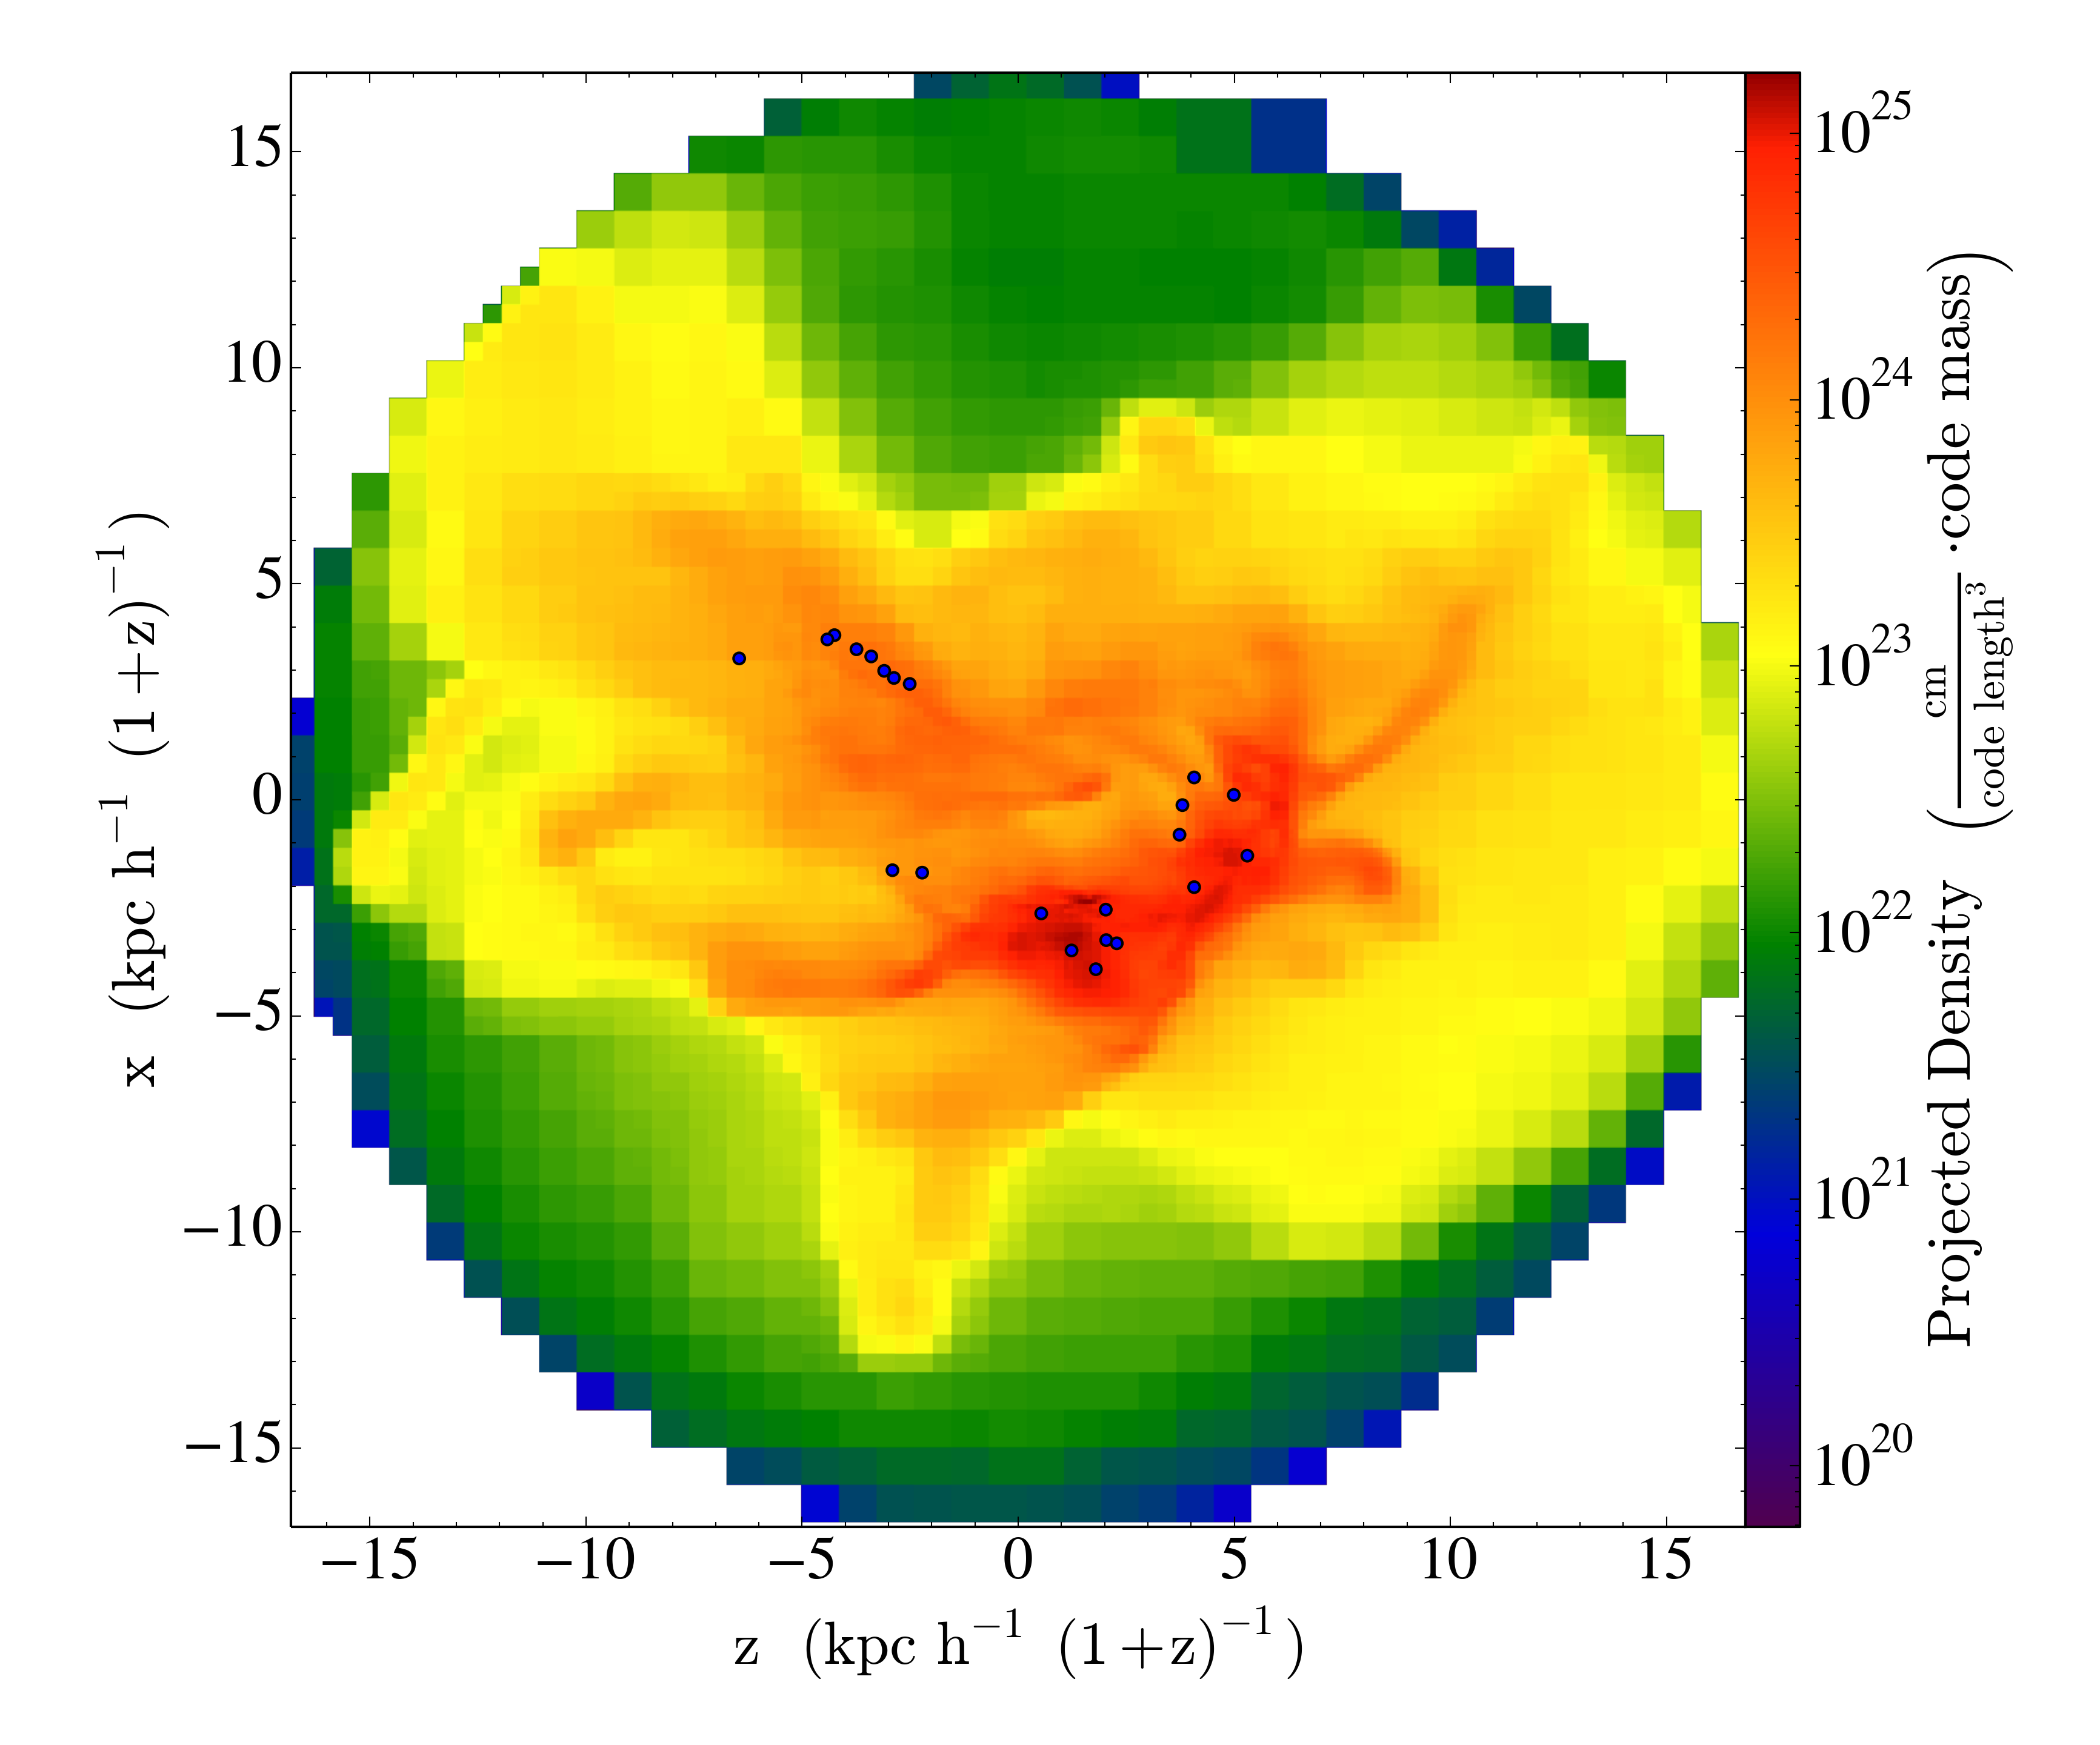
\includegraphics[width=0.8\columnwidth]{P0224_y_D.png}
\end{figure}

\begin{figure}
  \centering
  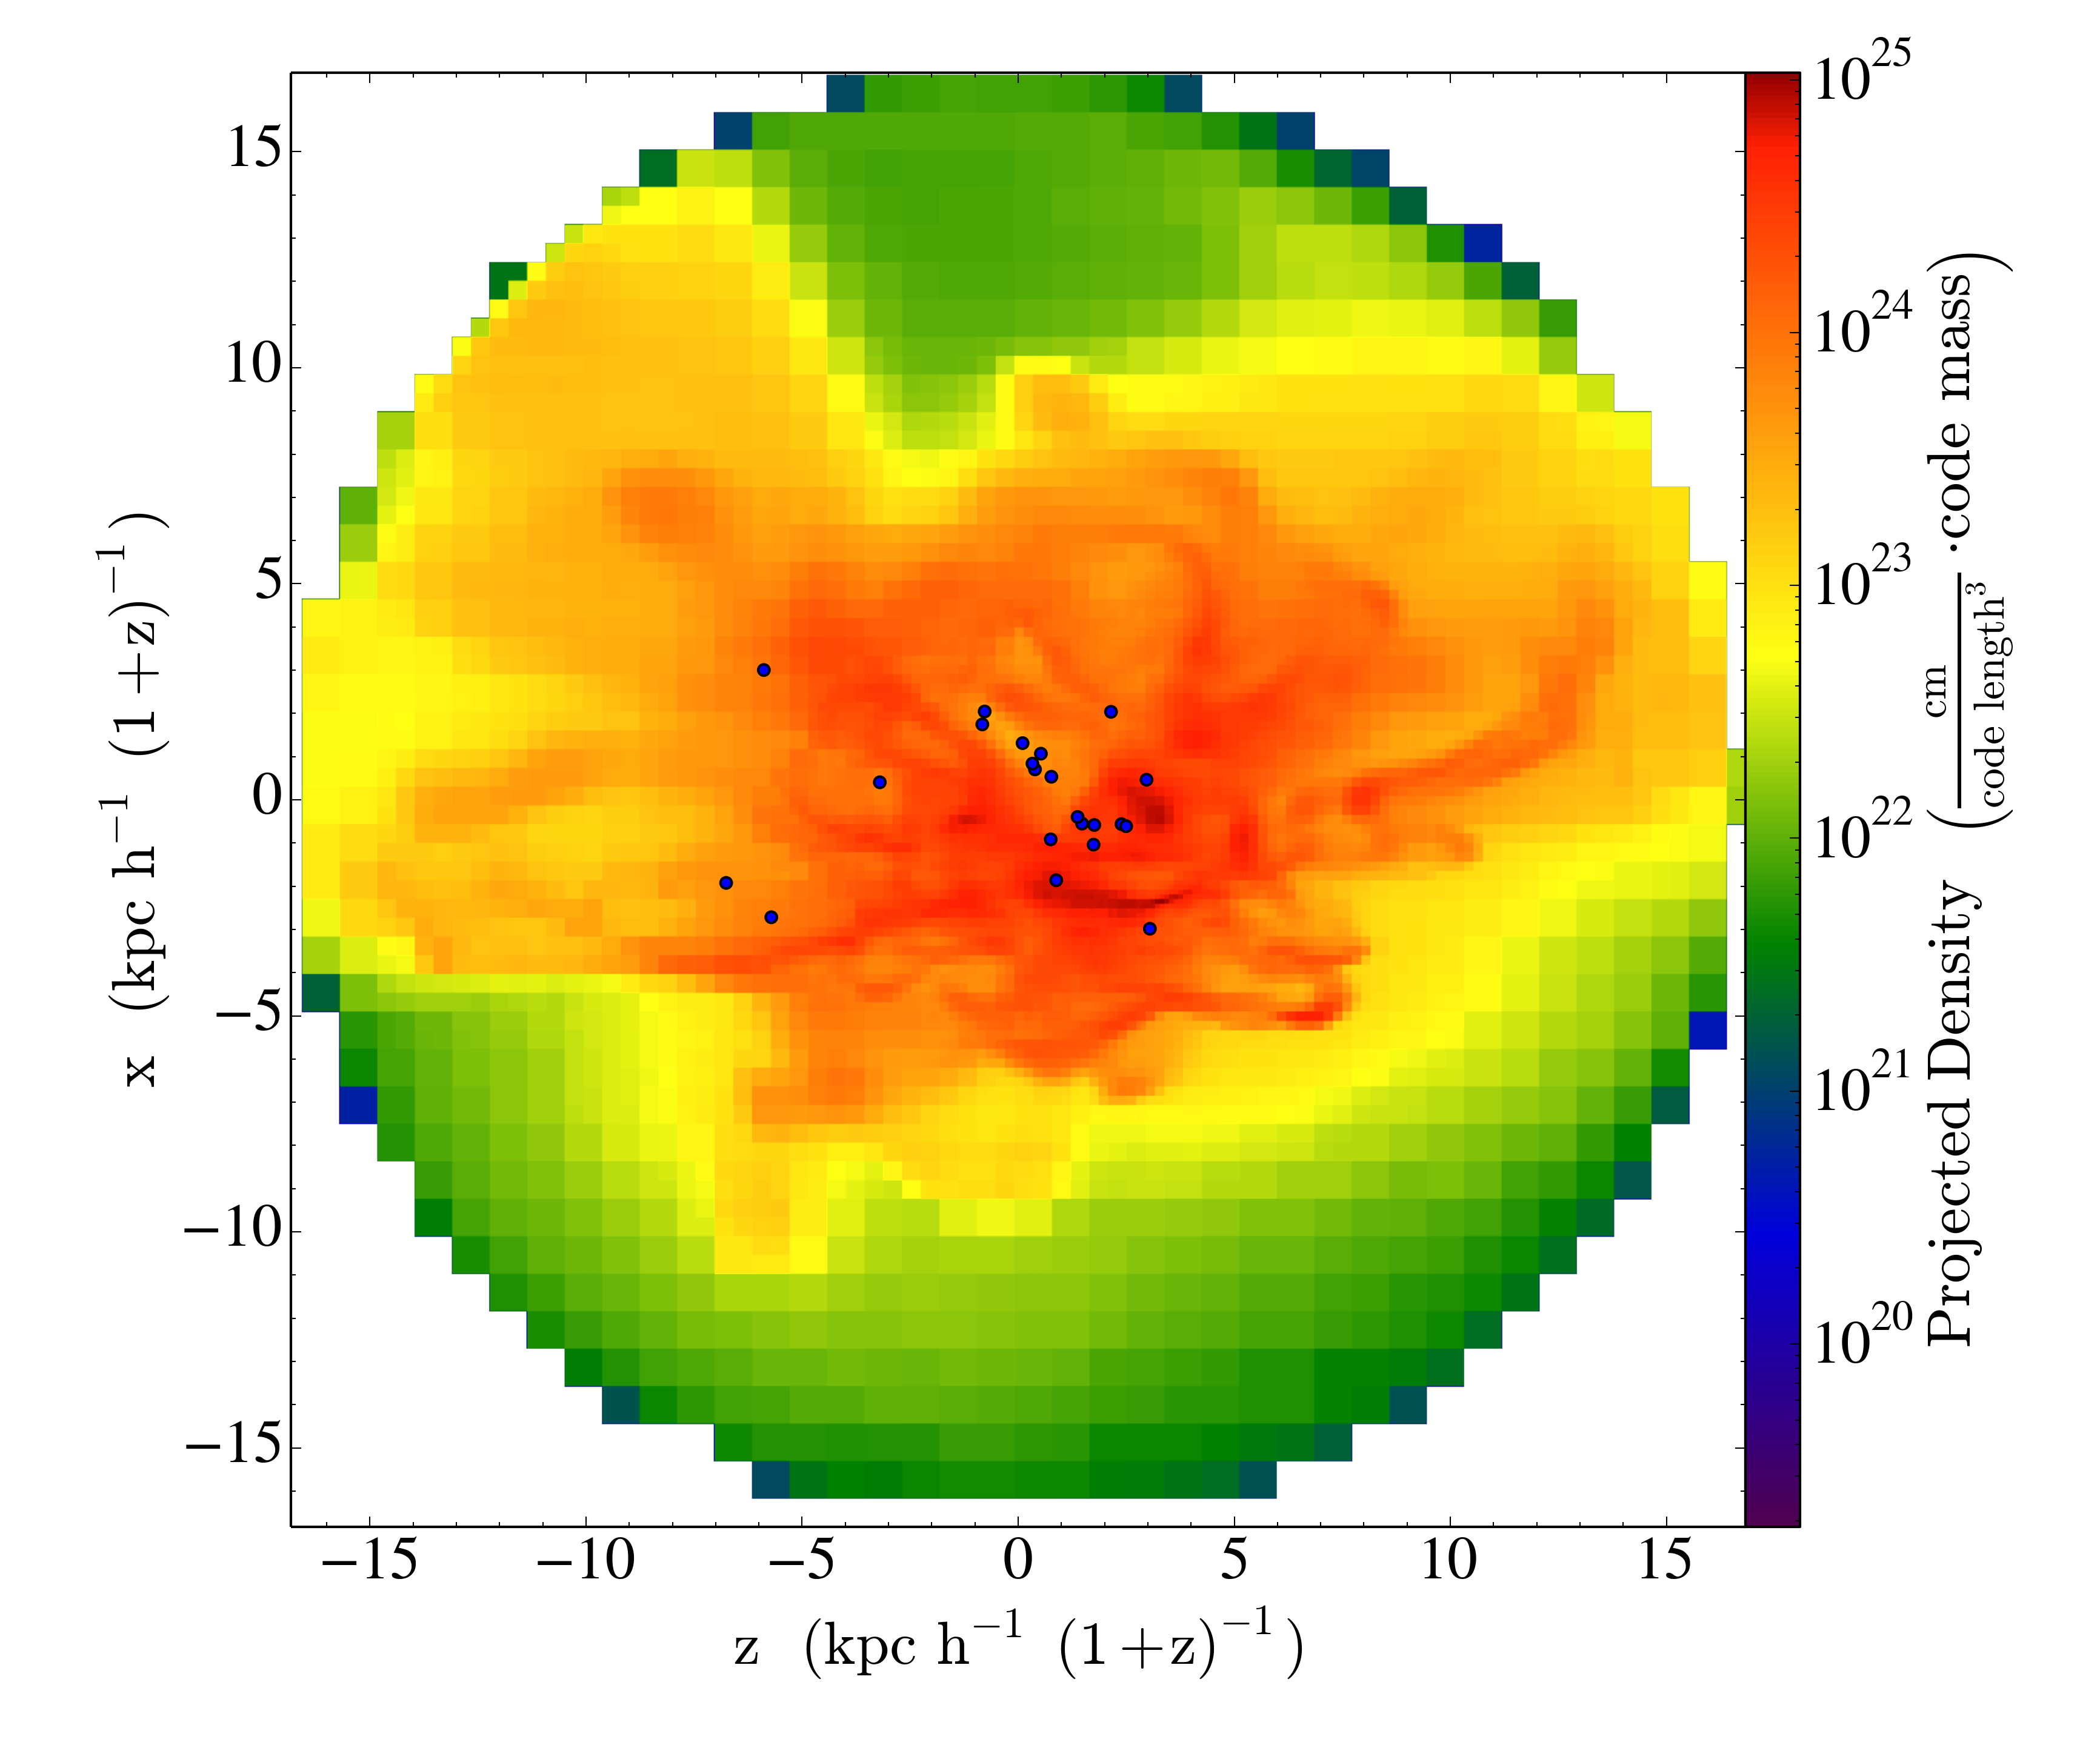
\includegraphics[width=0.8\columnwidth]{P0274_y_D.png}
\end{figure}
Angular momentum evolution:

\begin{figure}
  \centering
  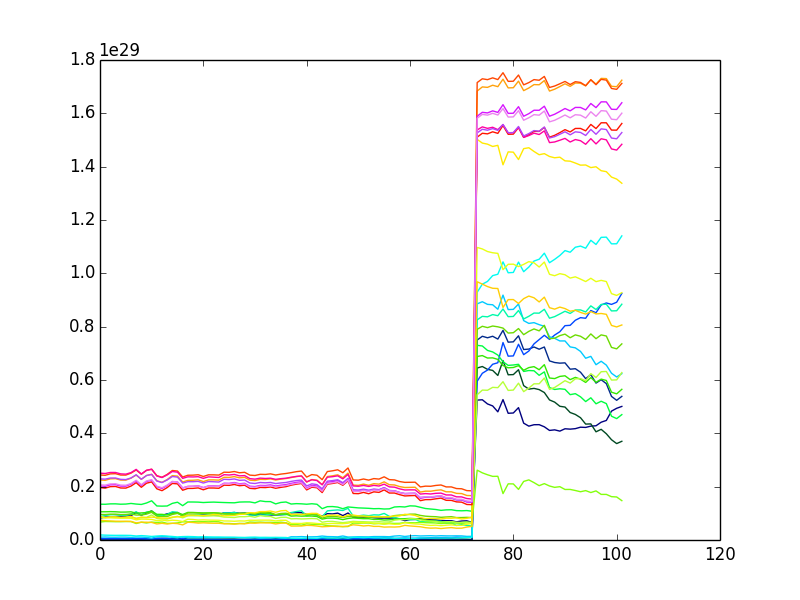
\includegraphics[width=0.8\columnwidth]{L2.png}
\end{figure}



\section*{Acknowledgments}

This work is supported by NSF grants AST-1211626 and AST-1333360.
This research has made use of NASA's Astrophysics Data System
Bibliographic Services.  The majority of the analysis and plots were
done with \yt~\citep{yt_full_paper}.

\bibliography{jwise}
\bsp
\label{lastpage}

\end{document}
